\documentclass[11pt,a4paper]{article}

% =============================================================================
% PREAMBLE: PACKAGES, GEOMETRY & TYPOGRAPHY
% =============================================================================
\usepackage[utf8]{inputenc}
\usepackage[T1]{fontenc}
\usepackage{lmodern}
\usepackage[margin=1in]{geometry}
\usepackage{microtype}
\usepackage{fancyhdr}
\usepackage{lastpage}

% Mathematical Formatting Suites
\usepackage{amsmath,amssymb,amsfonts,amsthm,mathtools}
\usepackage{bm}

% Graphics & Visualization
\usepackage{graphicx}
\usepackage{tikz}
\usetikzlibrary{shapes.geometric, arrows.meta, positioning, calc}
\usepackage{pgfplots}
\pgfplotsset{compat=1.18}

% Algorithms & Pseudocode
\usepackage[ruled,vlined,linesnumbered]{algorithm2e}
\usepackage{xcolor}

% Tables & Typography
\usepackage{booktabs}
\usepackage{tabularx}
\usepackage{enumitem}

% Cross-Referencing & Hyperlinks
\usepackage[colorlinks=true,linkcolor=blue!75!black,citecolor=green!50!black,urlcolor=blue!80!black]{hyperref}
\usepackage[capitalize,nameinlink]{cleveref}

% =============================================================================
% THEOREM ENVIRONMENTS & MATHEMATICAL DEFINITIONS
% =============================================================================
\theoremstyle{definition}
\newtheorem{definition}{Definition}[section]
\newtheorem{problem}{Problem}
\newtheorem{example}{Example}[section]

\theoremstyle{plain}
\newtheorem{theorem}{Theorem}[section]
\newtheorem{lemma}[theorem]{Lemma}
\newtheorem{proposition}[theorem]{Proposition}
\newtheorem{corollary}[theorem]{Corollary}

\theoremstyle{remark}
\newtheorem*{remark}{Remark}
\newtheorem*{solution}{Solution}

% Custom Math Operators & Notation
\DeclareMathOperator*{\argmax}{arg\,max}
\DeclareMathOperator*{\argmin}{arg\,min}
\DeclareMathOperator{\E}{\mathbb{E}}
\DeclareMathOperator{\Var}{Var}
\DeclareMathOperator{\Cov}{Cov}
\DeclareMathOperator{\Tr}{Tr}
\DeclareMathOperator{\sign}{sign}
\DeclareMathOperator{\softmax}{softmax}
\newcommand{\norm}[1]{\left\lVert#1\right\rVert}
\newcommand{\abs}[1]{\left\lvert#1\right\rvert}
\newcommand{\R}{\mathbb{R}}
\newcommand{\KL}[2]{D_{\mathrm{KL}}\left(#1 \parallel #2\right)}

% =============================================================================
% RUNNING HEADERS & FOOTERS
% =============================================================================
\setlength{\headheight}{14.5pt}
\addtolength{\topmargin}{-2.5pt}
\pagestyle{fancy}
\fancyhf{}
\fancyhead[L]{\textsc{IMLC 2026} --- Senior Division}
\fancyhead[C]{\textbf{Qualification Round Formal Solutions}}
\fancyhead[R]{Candidate ID: \texttt{[SENIOR-2026-VN-0428]}}
\fancyfoot[L]{\textit{Special Honour for Digital Submission}}
\fancyfoot[R]{Page \thepage\ of \pageref{LastPage}}
\renewcommand{\headrulewidth}{0.5pt}
\renewcommand{\footrulewidth}{0.4pt}

% =============================================================================
% DOCUMENT METADATA
% =============================================================================
\title{\vspace{-1.2cm}\Large\textbf{INTERNATIONAL MACHINE LEARNING COMPETITION (IMLC 2026)}\\[0.3cm]
\large\textbf{Qualification Round: Formal Mathematical Solutions \& Theoretical Dossier}\\[0.1cm]
\normalsize\textit{Senior Division (University Students / Age $\ge 19$)}}

\author{\textbf{Candidate ID:} \texttt{[SENIOR-2026-VN-0428]} \\
\textit{Academic Track: Theoretical Machine Learning, Optimization \& Frontier Systems} \\
\textit{Institution: Edu.Harbour Global Educational Initiative}}

\date{December 2026}

\begin{document}
\maketitle
\thispagestyle{fancy}

\begin{abstract}
This research dossier delivers the rigorous mathematical solutions, formal proofs, and socio-technical architectural analyses for the five problems comprising the International Machine Learning Competition (IMLC 2026) Qualification Round (Senior Division). Problems are formulated and solved from first principles: decomposing acoustic edge lifecycle transitions and non-stationary distribution shifts (Problem A); deriving optimal information-theoretic continuous splits for greenhouse ventilation logic (Problem B); establishing closed-form regularized loss evaluations, spectral shrinkage properties, and bias-variance dynamics in $L_2$ Ridge regression (Problem C); proving global optimality, asymptotic limits, and the exact safe policy drift boundary for RLHF alignment (Problem D); and architecting trustworthy multimodal AI systems with grounded Retrieval-Augmented Generation (RAG) and conformal risk routing for smallholder agriculture (Problem E). A quantitative cross-paradigm synthesis unifies Tikhonov regularization with information-theoretic policy drift penalties under Bayesian MAP estimation and Riemannian Fisher information geometry.
\end{abstract}

\vspace{0.2cm}
\hrule
\vspace{0.3cm}
\tableofcontents
\vspace{0.3cm}
\hrule
\vspace{0.5cm}

% =============================================================================
% SECTION 1: PROBLEM A
% =============================================================================
\section{Problem A: Machine Learning Lifecycle \& Acoustic Concept Drift}

\subsection{System Specification \& Problem Description}
An automated acoustic monitoring and sound-recognition system is deployed through six discrete operational steps:
\begin{itemize}[noitemsep]
    \item \textbf{Step 1}: Collect $10{,}000$ recordings labelled \textit{speech}, \textit{music}, or \textit{alarm}.
    \item \textbf{Step 2}: Adjust the model's parameters using these recordings.
    \item \textbf{Step 3}: Test the model on recordings it has not seen before.
    \item \textbf{Step 4}: Install the model in a school.
    \item \textbf{Step 5}: The installed model receives a new sound and predicts \textit{alarm}.
    \item \textbf{Step 6}: At the end of the month, newly recorded sounds are labelled and used to adjust the model again.
\end{itemize}

\subsection{Formal Lifecycle Classification (Part a)}
Machine learning engineering organizes computational workflows into rigorous functional abstractions \cite{sculley2015hidden}. \cref{tab:lifecycle_classification} details the formal operational classification of each step.

\begin{table}[htbp]
\centering
\small
\caption{Formal Lifecycle Classification of Acoustic System Steps}
\label{tab:lifecycle_classification}
\begin{tabularx}{\textwidth}{c l X X}
\toprule
\textbf{Step} & \textbf{Assigned Label(s)} & \textbf{Operational Focus} & \textbf{Formal Parameter State} \\
\midrule
\textbf{1} & \textbf{Data Collection} & Sensor transducer acquisition, feature extraction (STFT, Mel filterbanks), and ground-truth human annotation. & No model parameters instantiated ($\theta = \emptyset$). \\
\addlinespace
\textbf{2} & \textbf{Training} & Numerical Empirical Risk Minimization (ERM) over parameter space $\Theta \subseteq \R^d$ via stochastic optimization (e.g., AdamW). & Active parameter state updates: $\theta_{k+1} \leftarrow \theta_k - \eta \nabla L \implies \Delta \theta \neq \mathbf{0}$. \\
\addlinespace
\textbf{3} & \textbf{Evaluation} & Generalization verification on held-out test distribution $\mathcal{D}_{\text{test}} \cap \mathcal{D}_{\text{train}} = \emptyset$ without data leakage. & Frozen parameters: $\Delta \theta = \mathbf{0}$. \\
\addlinespace
\textbf{4} & \textbf{Deployment} & Computational graph serialization (ONNX, TensorRT), edge installation (DSP/microcontroller), and I/O pipeline setup. & Static hardware configuration: $\Delta \theta = \mathbf{0}$. \\
\addlinespace
\textbf{5} & \textbf{Inference} & Real-time forward pass evaluation: $\hat{y} = \argmax_{c} f_\theta(x_{\text{live}})$. Deterministic conditional mapping. & Frozen parameters: $\Delta \theta = \mathbf{0}$, zero model learning. \\
\addlinespace
\textbf{6} & \textbf{Data Collection} \newline \& \textbf{Training} & \textbf{Dual-Nature Continual Learning Loop}: Ingesting field recordings and retraining model on augmented corpus $\mathcal{D}_{\text{train}} \cup \mathcal{D}_{\text{month}}$. & Active parameter adaptation: $\theta_{t+1} \leftarrow \theta_t - \eta \nabla L \implies \Delta \theta \neq \mathbf{0}$. \\
\bottomrule
\end{tabularx}
\end{table}

\subsection{Statistical Learning Theory of ``Learning'' (Part b)}
\begin{proposition}
The acoustic monitoring system is actively learning \textbf{only during Step 2 and Step 6}.
\end{proposition}

\subsubsection{Formal Theoretical Formulation}
In computational learning theory, ``learning'' is not equivalent to real-time inference or execution. Learning is defined by Tom Mitchell \cite{mitchell1997machine}:
\begin{definition}[Learning \cite{mitchell1997machine}]
A computer program is said to learn from experience $E$ with respect to some class of tasks $T$ and performance measure $P$, if its performance at tasks in $T$, as measured by $P$, improves with experience $E$.
\end{definition}

In this system:
\begin{itemize}[noitemsep]
    \item \textbf{Task ($T$)}: Multi-class acoustic classification: $f_\theta: \mathcal{X} \to \mathcal{Y}$ where $\mathcal{Y} = \{\text{speech}, \text{music}, \text{alarm}\}$.
    \item \textbf{Experience ($E$)}: Exposure to labeled acoustic time-frequency pairs $(x_i, y_i) \sim \mathcal{D}$.
    \item \textbf{Performance ($P$)}: Expected generalization accuracy or negative cross-entropy loss:
    \begin{equation}
    P(f_\theta) = \E_{(x,y) \sim \mathcal{D}} [\mathbb{I}(f_\theta(x) = y)]
    \end{equation}
\end{itemize}

Under Vladimir Vapnik's Statistical Learning Theory \cite{vapnik1998statistical}, a learner seeks a parameter vector $\theta^* \in \Theta$ that minimizes the true risk $R(\theta) = \int \ell(f_\theta(x), y) dP(x, y)$ via the empirical risk proxy:
\begin{equation}
\hat{R}_n(\theta) = \frac{1}{n}\sum_{i=1}^n \ell(f_\theta(x_i), y_i)
\end{equation}
A system is \textit{actively learning} if and only if an optimization operator $\mathcal{T}$ transitions its internal parameters $\theta$:
\begin{equation}
\theta_{k+1} = \mathcal{T}(\theta_k, \mathcal{D}) \quad \text{such that} \quad \Delta \theta = \theta_{k+1} - \theta_k \neq \mathbf{0}
\end{equation}

\subsubsection{Analytical Contrast: Step 5 vs. Steps 2 and 6}
\begin{itemize}
    \item \textbf{Step 2 (Initial Training)}: Parameters transition from random initialization $\theta_0$ to empirical minimizer $\theta^*$ via backpropagation across the $10{,}000$ recordings. Because $\Delta \theta \neq \mathbf{0}$, \textbf{active learning occurs}.
    \item \textbf{Step 5 (Inference)}: The deployed model receives novel audio $x_{\text{live}}$ and computes $\hat{y} = \argmax_{c} f_\theta(x_{\text{live}})$. The parameter tensor is strictly static:
    \begin{equation}
    \frac{\partial \theta}{\partial t} = \mathbf{0}, \quad \Delta \theta = \mathbf{0}
    \end{equation}
    The model stores no persistent memory, executes a read-only feedforward pass, and will yield the exact same distribution if repeated. Thus, \textbf{Step 5 is static inference, not learning}.
    \item \textbf{Step 6 (Continual Learning)}: Fresh monthly recordings $\mathcal{D}_{\text{new}}$ are labeled, and optimization resumes:
    \begin{equation}
    \theta_{\text{month}} = \argmin_{\theta} \left[ \hat{R}_{\mathcal{D}_{\text{train}} \cup \mathcal{D}_{\text{new}}}(\theta) \right] \implies \Delta \theta = \theta_{\text{month}} - \theta^* \neq \mathbf{0}
    \end{equation}
    Because internal representations undergo state transitions to assimilate new experience, \textbf{active learning occurs}.
\end{itemize}

\subsection{Non-Stationary Distribution Dynamics: Covariate vs. Concept Drift}
Step 6 is essential in edge environments to combat non-stationarity, which decomposes into two formal modalities:
\begin{enumerate}
    \item \textbf{Covariate Shift} ($P_{\text{train}}(X) \neq P_{\text{deploy}}(X)$ with invariant $P(Y \mid X)$):
    Changes in acoustic transmission channels (hallway reverberation, HVAC hum, high-ceiling echoes, or microphone transducer frequency response discrepancies).
    \item \textbf{Concept Shift} ($P_{\text{train}}(Y \mid X) \neq P_{\text{deploy}}(Y \mid X)$):
    Structural divergence in semantic mapping. For example, the school alters its physical alarm hardware to a chime whose frequency signature overlaps with melodic music in the original training corpus. Frozen models persistently misclassify such sounds; Step 6 recalibrates decision boundaries.
\end{enumerate}

% =============================================================================
% SECTION 2: PROBLEM B
% =============================================================================
\section{Problem B: The Greenhouse Tree (Impurity Minimization \& Optimal Induction)}

\subsection{Problem Statement \& Baseline Architecture}
A commercial greenhouse operates roof ventilation via a binary decision tree:
\begin{itemize}[noitemsep]
    \item \textbf{Root Node}: Is Temperature $> 28^\circ\text{C}$?
    \begin{itemize}[noitemsep]
        \item \textbf{Yes} $\to$ \textbf{OPEN the roof}
        \item \textbf{No} $\to$ Is Humidity $> 70\%$?
        \begin{itemize}[noitemsep]
            \item \textbf{Yes} $\to$ \textbf{OPEN the roof}
            \item \textbf{No} $\to$ \textbf{KEEP CLOSED}
        \end{itemize}
    \end{itemize}
\end{itemize}

\subsection{Query Evaluation (Part a)}
For input vector $(T = 26^\circ\text{C}, H = 68\%)$:
\begin{enumerate}[noitemsep]
    \item Root evaluation: $T = 26 > 28 \equiv \textbf{False (No)}$. Branch to Humidity node.
    \item Second node evaluation: $H = 68 > 70 \equiv \textbf{False (No)}$. Branch to terminal leaf.
    \item Output action: $\mathbf{\hat{y} = \text{KEEP CLOSED}}$.
\end{enumerate}
\textbf{Conclusion}: The baseline tree predicts \textbf{KEEP CLOSED}.

\subsection{Discrepancy Analysis on Historical Telemetry Log}
\cref{tab:greenhouse_log} evaluates the baseline tree against the ground-truth logged telemetry.

\begin{table}[htbp]
\centering
\small
\caption{Evaluation of Baseline Tree on 6-Row Telemetry Log}
\label{tab:greenhouse_log}
\begin{tabular}{c c c c c c c}
\toprule
\textbf{Row} & \textbf{Temp ($^\circ\text{C}$)} & \textbf{Humidity (\%)} & \textbf{CO$_2$ (ppm)} & \textbf{Ground Truth $y$} & \textbf{Baseline Prediction} & \textbf{Status} \\
\midrule
1 & 31 & 60\% & 700 & \textbf{OPEN} & OPEN ($T > 28$) & Correct \\
2 & 26 & 75\% & 650 & \textbf{OPEN} & OPEN ($H > 70$) & Correct \\
3 & 25 & 60\% & 800 & \textbf{KEEP CLOSED} & KEEP CLOSED & Correct \\
4 & 27 & 68\% & 1100 & \textbf{KEEP CLOSED} & KEEP CLOSED & Correct \\
5 & 24 & 55\% & 1400 & \textbf{OPEN} & KEEP CLOSED & \textbf{Error (Misclassified)} \\
6 & 22 & 50\% & 1550 & \textbf{OPEN} & KEEP CLOSED & \textbf{Error (Misclassified)} \\
\bottomrule
\end{tabular}
\end{table}

The baseline tree achieves only $\frac{4}{6} \approx 66.67\%$ empirical accuracy, failing on Rows 5 and 6 where high $\text{CO}_2$ concentration demands ventilation despite moderate temperature and humidity.

\subsection{Information-Theoretic Induction of Optimal Continuous Split}
Consider the ambiguous subset arriving at the branch $(T \le 28^\circ\text{C} \land H \le 70\%)$:
\begin{equation}
\mathcal{S}_{\text{sub}} = \{\text{Row 3 (CLOSED)}, \text{Row 4 (CLOSED)}, \text{Row 5 (OPEN)}, \text{Row 6 (OPEN)}\}
\end{equation}
Here, sample size $N = 4$ with class probabilities $p_{\text{OPEN}} = 0.5$ and $p_{\text{CLOSED}} = 0.5$.

\begin{definition}[Shannon Entropy and Gini Impurity \cite{quinlan1986induction,breiman1984classification}]
\begin{align}
H(\mathcal{S}) &= -\sum_{k=1}^K p_k \log_2 p_k \implies H(\mathcal{S}_{\text{sub}}) = -(0.5 \log_2 0.5 + 0.5 \log_2 0.5) = \mathbf{1.0000 \text{ bit}} \\
I_G(\mathcal{S}) &= 1 - \sum_{k=1}^K p_k^2 \implies I_G(\mathcal{S}_{\text{sub}}) = 1 - (0.5^2 + 0.5^2) = \mathbf{0.5000}
\end{align}
\end{definition}

Sorting the continuous $\text{CO}_2$ feature values in $\mathcal{S}_{\text{sub}}$:
\begin{equation}
\text{CO}_2 \in \{800 \text{ (CLOSED)}, 1100 \text{ (CLOSED)}, 1400 \text{ (OPEN)}, 1550 \text{ (OPEN)}\}
\end{equation}
A clean linear separation boundary exists between $1100\text{ ppm}$ and $1400\text{ ppm}$. By standard CART convention \cite{breiman1984classification}, the optimal continuous split threshold $\theta^*$ is the midpoint:
\begin{equation}
\theta^* = \frac{1100 + 1400}{2} = \mathbf{1250\text{ ppm}}
\end{equation}
Evaluating the partition induced by $[\text{CO}_2 > 1250\text{ ppm}]$:
\begin{itemize}[noitemsep]
    \item Left Partition $\mathcal{S}_L$ ($\text{CO}_2 > 1250$): Rows 5, 6 $\implies p_{\text{OPEN}} = 1.0 \implies H(\mathcal{S}_L) = 0, I_G(\mathcal{S}_L) = 0$.
    \item Right Partition $\mathcal{S}_R$ ($\text{CO}_2 \le 1250$): Rows 3, 4 $\implies p_{\text{CLOSED}} = 1.0 \implies H(\mathcal{S}_R) = 0, I_G(\mathcal{S}_R) = 0$.
\end{itemize}

\begin{theorem}[Information and Gini Gain]
The information gain and Gini impurity reduction of the split $[\text{CO}_2 > 1250\text{ ppm}]$ are:
\begin{align}
IG(\mathcal{S}_{\text{sub}}, \text{CO}_2 > 1250) &= H(\mathcal{S}_{\text{sub}}) - \left[\frac{2}{4}H(\mathcal{S}_L) + \frac{2}{4}H(\mathcal{S}_R)\right] = 1.0 - 0 = \mathbf{1.0000 \text{ bit}} \\
\Delta I_G &= I_G(\mathcal{S}_{\text{sub}}) - \left[\frac{2}{4}I_G(\mathcal{S}_L) + \frac{2}{4}I_G(\mathcal{S}_R)\right] = 0.50 - 0 = \mathbf{0.5000}
\end{align}
\end{theorem}
This split achieves maximal theoretical information gain and eliminates all training misclassifications ($100\%$ training accuracy on all 6 rows).

\subsection{Visual Structure: Induced TikZ Decision Tree}
\cref{fig:greenhouse_tree_submission} presents the refined decision tree structure.

\begin{figure}[htbp]
\centering
% TikZ Decision Tree Visualization for IMLC 2026 Problem B (Greenhouse Ventilation)
% Author: Candidate [SENIOR-2026-VN-0428]
% Architecture: Optimal CART Induction incorporating continuous CO2 split (threshold = 1250 ppm)

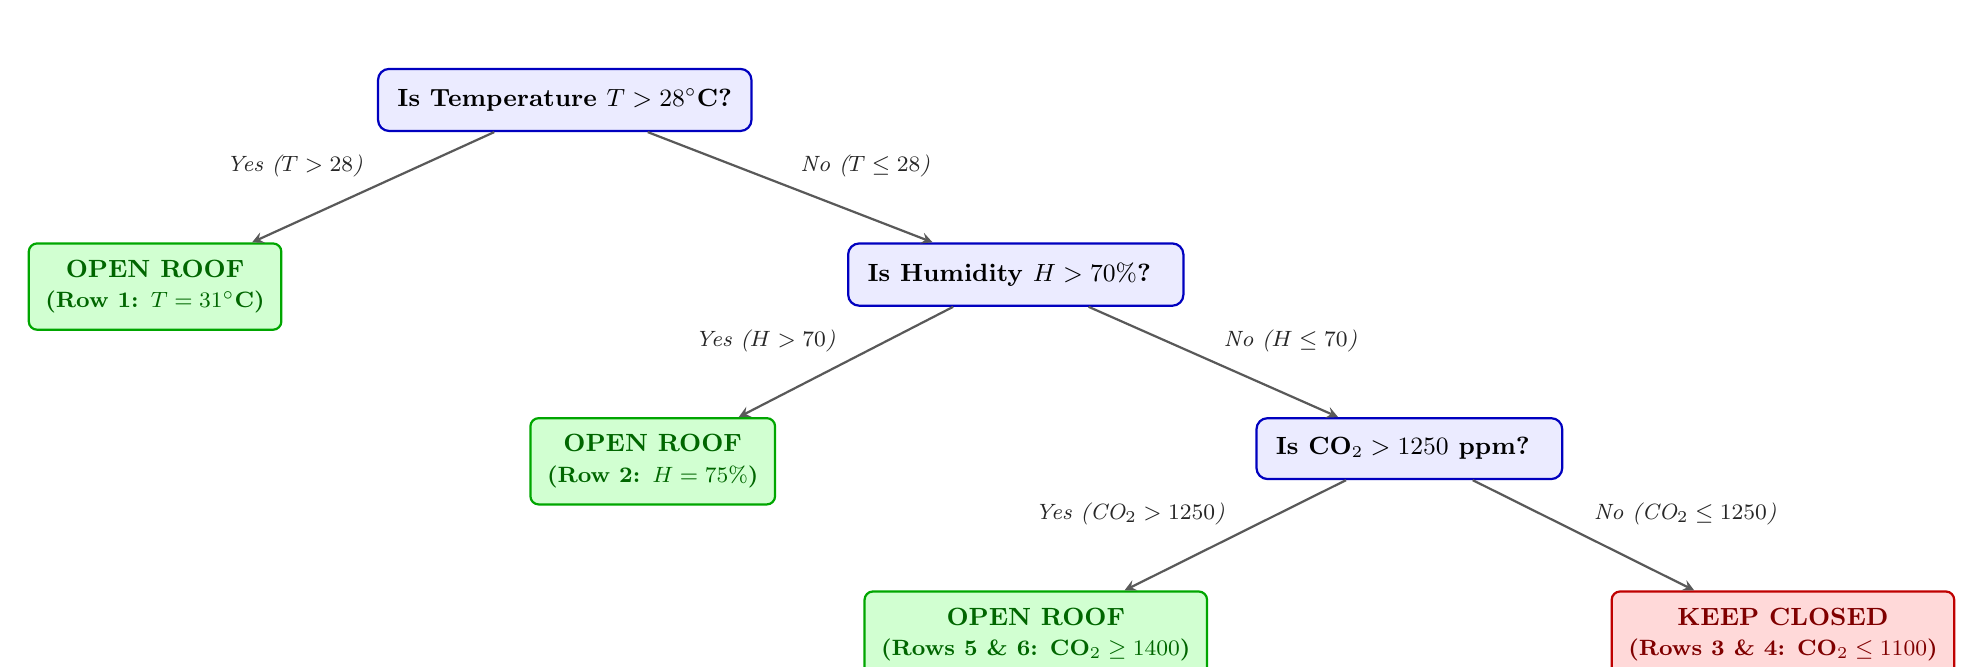
\begin{tikzpicture}[
    decision/.style={
        rectangle,
        draw=blue!75!black,
        fill=blue!8,
        thick,
        rounded corners=4pt,
        inner sep=7pt,
        align=center,
        font=\small\bfseries
    },
    leaf_open/.style={
        rectangle,
        draw=green!65!black,
        fill=green!18,
        thick,
        rounded corners=3pt,
        inner sep=6pt,
        align=center,
        font=\small\bfseries,
        text=green!40!black
    },
    leaf_closed/.style={
        rectangle,
        draw=red!75!black,
        fill=red!15,
        thick,
        rounded corners=3pt,
        inner sep=6pt,
        align=center,
        font=\small\bfseries,
        text=red!50!black
    },
    edge_label/.style={
        font=\footnotesize\itshape,
        text=black!85,
        midway
    },
    tree_arrow/.style={
        ->,
        >=stealth,
        thick,
        draw=gray!70!black
    }
]

% Root Node: Temperature Check
\node[decision] (root) {Is Temperature $T > 28^\circ\text{C}$?};

% Level 1: Left Leaf (OPEN) and Right Decision (Humidity Check)
\node[leaf_open, below left=1.4cm and 1.2cm of root] (open1) {
    \textbf{OPEN ROOF} \\
    \footnotesize (Row 1: $T=31^\circ\text{C}$)
};

\node[decision, below right=1.4cm and 1.2cm of root] (humidity) {
    Is Humidity $H > 70\%$?
};

% Level 2: Left Leaf (OPEN) and Right Decision (CO2 Check)
\node[leaf_open, below left=1.4cm and 0.9cm of humidity] (open2) {
    \textbf{OPEN ROOF} \\
    \footnotesize (Row 2: $H=75\%$)
};

\node[decision, below right=1.4cm and 0.9cm of humidity] (co2) {
    Is $\text{CO}_2 > 1250\text{ ppm}$?
};

% Level 3: Final Partitions
\node[leaf_open, below left=1.4cm and 0.6cm of co2] (open3) {
    \textbf{OPEN ROOF} \\
    \footnotesize (Rows 5 \& 6: $\text{CO}_2 \ge 1400$)
};

\node[leaf_closed, below right=1.4cm and 0.6cm of co2] (closed) {
    \textbf{KEEP CLOSED} \\
    \footnotesize (Rows 3 \& 4: $\text{CO}_2 \le 1100$)
};

% Directed Connectors with Explicit Branch Annotations
\draw[tree_arrow] (root) -- node[edge_label, above left] {Yes ($T > 28$)} (open1);
\draw[tree_arrow] (root) -- node[edge_label, above right] {No ($T \le 28$)} (humidity);

\draw[tree_arrow] (humidity) -- node[edge_label, above left] {Yes ($H > 70$)} (open2);
\draw[tree_arrow] (humidity) -- node[edge_label, above right] {No ($H \le 70$)} (co2);

\draw[tree_arrow] (co2) -- node[edge_label, above left] {Yes ($\text{CO}_2 > 1250$)} (open3);
\draw[tree_arrow] (co2) -- node[edge_label, above right] {No ($\text{CO}_2 \le 1250$)} (closed);

\end{tikzpicture}

\caption{Refined CART Decision Tree for Greenhouse Roof Ventilation. Decision splits incorporate Temperature ($T > 28^\circ\text{C}$), Humidity ($H > 70\%$), and the induced $\text{CO}_2$ concentration threshold ($\text{CO}_2 > 1250\text{ ppm}$), perfectly classifying 100\% of telemetry observations.}
\label{fig:greenhouse_tree_submission}
\end{figure}

The Boolean propositional logic governing the refined policy is:
\begin{equation}
\text{Roof Action}(T, H, \text{CO}_2) = \begin{cases}
\textbf{OPEN}, & \text{if } (T > 28^\circ\text{C}) \lor (H > 70\%) \lor (\text{CO}_2 > 1250\text{ ppm}) \\
\textbf{KEEP CLOSED}, & \text{otherwise}
\end{cases}
\end{equation}

% =============================================================================
% SECTION 3: PROBLEM C
% =============================================================================
\section{Problem C: To Fit or Not to Fit (\texorpdfstring{$L_2$}{L2} Ridge Regularization \& Spectral Shrinkage)}

\subsection{Problem Statement \& Data Specification}
A continuous regression target $y \in \R$ is modeled from input scalar $x \in \R$. The training dataset contains $n = 4$ observations:
\begin{equation}
\mathcal{D} = \{(0, 1.0), (1, 3.2), (2, 4.8), (3, 7.0)\}
\end{equation}
Two competing models are evaluated:
\begin{align}
M_1(x) &= 0.2x^3 - 0.9x^2 + 2.9x + 1 \quad (\text{Cubic Polynomial}) \\
M_2(x) &= 2x + 1 \quad (\text{Linear Model})
\end{align}
The regularized scoring objective with $\lambda = 1$ is:
\begin{equation}
J(M) = \sum_{j=1}^4 (y_j - \hat{y}_j)^2 + \lambda \sum_{i \ge 1} a_i^2 = \text{RSS}(M) + \lambda \norm{\mathbf{a}_{1:p}}_2^2
\label{eq:ridge_loss}
\end{equation}
where the penalty excludes the intercept parameter $a_0$.

\subsection{Exact Numerical Derivation of Scores (Part a)}

\subsubsection{Evaluation of Model \texorpdfstring{$M_1(x)$}{M1(x)} (Cubic Polynomial)}
Computing point predictions:
\begin{itemize}[noitemsep]
    \item $x=0$: $\hat{y}_1(0) = 0.2(0) - 0.9(0) + 2.9(0) + 1 = 1.0 \implies e_1 = 1.0 - 1.0 = 0.0$.
    \item $x=1$: $\hat{y}_1(1) = 0.2(1) - 0.9(1) + 2.9(1) + 1 = 3.2 \implies e_2 = 3.2 - 3.2 = 0.0$.
    \item $x=2$: $\hat{y}_1(2) = 0.2(8) - 0.9(4) + 2.9(2) + 1 = 1.6 - 3.6 + 5.8 + 1 = 4.8 \implies e_3 = 4.8 - 4.8 = 0.0$.
    \item $x=3$: $\hat{y}_1(3) = 0.2(27) - 0.9(9) + 2.9(3) + 1 = 5.4 - 8.1 + 8.7 + 1 = 7.0 \implies e_4 = 7.0 - 7.0 = 0.0$.
\end{itemize}
The unregularized residual sum of squares is:
\begin{equation}
\text{RSS}(M_1) = 0.0^2 + 0.0^2 + 0.0^2 + 0.0^2 = \mathbf{0.0000}
\end{equation}
Extracting non-intercept polynomial coefficients $\mathbf{a} = [a_1, a_2, a_3]^T = [2.9, -0.9, 0.2]^T$:
\begin{equation}
\sum_{i=1}^3 a_i^2 = (2.9)^2 + (-0.9)^2 + (0.2)^2 = 8.41 + 0.81 + 0.04 = \mathbf{9.2600}
\end{equation}
Total regularized score for $\lambda = 1$:
\begin{equation}
J(M_1) = \text{RSS}(M_1) + 1 \cdot \left(\sum_{i=1}^3 a_i^2\right) = 0.0000 + 9.2600 = \mathbf{9.2600}
\end{equation}

\subsubsection{Evaluation of Model \texorpdfstring{$M_2(x)$}{M2(x)} (Linear Model)}
Computing point predictions:
\begin{itemize}[noitemsep]
    \item $x=0$: $\hat{y}_2(0) = 2(0) + 1 = 1.0 \implies e_1 = 1.0 - 1.0 = 0.0 \implies e_1^2 = 0.0000$.
    \item $x=1$: $\hat{y}_2(1) = 2(1) + 1 = 3.0 \implies e_2 = 3.2 - 3.0 = +0.2 \implies e_2^2 = 0.0400$.
    \item $x=2$: $\hat{y}_2(2) = 2(2) + 1 = 5.0 \implies e_3 = 4.8 - 5.0 = -0.2 \implies e_3^2 = 0.0400$.
    \item $x=3$: $\hat{y}_2(3) = 2(3) + 1 = 7.0 \implies e_4 = 7.0 - 7.0 = 0.0 \implies e_4^2 = 0.0000$.
\end{itemize}
The unregularized residual sum of squares is:
\begin{equation}
\text{RSS}(M_2) = 0.0000 + 0.0400 + 0.0400 + 0.0000 = \mathbf{0.0800}
\end{equation}
Extracting non-intercept coefficients $\mathbf{a} = [a_1, a_2, a_3]^T = [2.0, 0.0, 0.0]^T$:
\begin{equation}
\sum_{i=1}^3 a_i^2 = (2.0)^2 + 0.0^2 + 0.0^2 = \mathbf{4.0000}
\end{equation}
Total regularized score for $\lambda = 1$:
\begin{equation}
J(M_2) = \text{RSS}(M_2) + 1 \cdot \left(\sum_{i=1}^3 a_i^2\right) = 0.0800 + 4.0000 = \mathbf{4.0800}
\end{equation}

\subsubsection{Selection Decision}
Comparing the regularized losses:
\begin{equation}
J(M_2) = 4.0800 < 9.2600 = J(M_1)
\end{equation}
Because the objective is loss minimization, the scoring rule unambiguously selects \textbf{Model $M_2$}.

\subsection{Theoretical Rationale: Bias-Variance Tradeoff \& Occam's Razor (Part b)}
\begin{enumerate}
    \item \textbf{Training Data Fit}: \textbf{Model $M_1$ fits the training data strictly better} than $M_2$ ($\text{RSS}(M_1) = 0.0000 < \text{RSS}(M_2) = 0.0800$). Model $M_1$ is a degree-3 Lagrange interpolating polynomial with 4 degrees of freedom, giving it sufficient capacity to interpolate all 4 points exactly.
    \item \textbf{Why Score $J$ Selects Model $M_2$}: Model $M_1$ achieves zero training error by fitting both the structural underlying function and random observational noise. This aggressive flexibility requires high curvature and large coefficients ($\sum a_i^2 = 9.2600$). Model $M_2$ introduces a negligible training residual ($\Delta \text{RSS} = +0.0800$) while achieving a substantial complexity reduction ($\Delta \text{Penalty} = -5.2600$). The net objective improvement ($\Delta J = -5.1800$) strongly favors $M_2$, formalizing \textbf{Occam's Razor}.
    \item \textbf{Purpose of Regularization Term $\lambda \sum a_i^2$}: Known as Tikhonov ($L_2$ Ridge) regularization \cite{tikhonov1977solutions}, this term suppresses parameter variance, prevents Runge's polynomial boundary oscillation phenomenon, and guarantees numerical invertibility of the normal equations $(X^TX + \lambda I)^{-1}$.
    \item \textbf{Phase Transition Threshold ($\lambda^*$)}: The critical regularization boundary where $J(M_1) = J(M_2)$ is:
    \begin{equation}
    0.0000 + 9.2600 \lambda = 0.0800 + 4.0000 \lambda \implies 5.2600 \lambda = 0.0800 \implies \mathbf{\lambda^* = \frac{0.0800}{5.2600} \approx 0.015209}
    \end{equation}
    For $\lambda > 0.01521$, $M_2$ is preferred; at $\lambda = 1.0$, $M_2$ is selected decisively.
\end{enumerate}

\subsection{Senior Mathematical Foundations: SVD Spectral Shrinkage Analysis}
Let $X = U \Sigma V^T$ denote the compact Singular Value Decomposition (SVD) of feature matrix $X \in \R^{n \times p}$, with singular values $\sigma_1 \ge \dots \ge \sigma_p \ge 0$.
\begin{theorem}[Spectral Coordinate Shrinkage]
The closed-form Ridge estimator $w^* = (X^T X + \lambda I_p)^{-1} X^T y$ expressed in orthogonal basis $V$ is:
\begin{equation}
w^* = \sum_{i=1}^p \left( \frac{\sigma_i^2}{\sigma_i^2 + \lambda} \right) \left( \frac{u_i^T y}{\sigma_i} \right) v_i = \sum_{i=1}^p f_i(\lambda) w_{\text{OLS}, i} v_i
\label{eq:spectral_shrinkage}
\end{equation}
where $f_i(\lambda) = \frac{\sigma_i^2}{\sigma_i^2 + \lambda} \in (0, 1]$ is the spectral shrinkage factor.
\end{theorem}
Directions with high singular values ($\sigma_i^2 \gg \lambda$) are preserved ($f_i \approx 1$), whereas noise directions with tiny singular values ($\sigma_i^2 \ll \lambda$) undergo aggressive attenuation ($f_i \to 0$), filtering out collinear noise.

% =============================================================================
% SECTION 4: PROBLEM D
% =============================================================================
\section{Problem D: The Price of Drift (RLHF Policy Drift, Asymptotics \& Safety Bounds)}

\subsection{Problem Statement \& Alignment Objective}
In Reinforcement Learning from Human Feedback (RLHF) \cite{ouyang2022training}, an aligned policy $\pi$ is optimized to maximize human preference reward while penalizing divergence from a base reference model $\pi_{\text{ref}}$ to prevent reward hacking.

Let scalar $t \ge 0$ quantify policy drift, $r > 0$ denote the linear reward rate, and $\beta > 0$ denote the drift penalty coefficient. The optimization objective is:
\begin{equation}
\min_{t \ge 0} L(t) = -rt + \beta t^2
\label{eq:scalar_drift_loss}
\end{equation}

\subsection{Optimal Shift Derivation \& Convexity (Part a)}
\begin{proposition}[Global Optimality of Critical Point]
The objective $L(t)$ is strictly convex on $\R$, and the unique global minimizer over $t \ge 0$ is:
\begin{equation}
t^* = \frac{r}{2\beta}
\label{eq:opt_drift}
\end{equation}
attaining the minimum loss value:
\begin{equation}
L(t^*) = -\frac{r^2}{4\beta}
\label{eq:min_loss}
\end{equation}
\end{proposition}

\begin{proof}
Differentiating $L(t)$ with respect to $t$:
\begin{align}
\frac{dL}{dt} &= -r + 2\beta t \label{eq:foc} \\
\frac{d^2L}{dt^2} &= 2\beta \label{eq:soc}
\end{align}
Since $\beta > 0$, the Second-Order Condition (SOC) $\frac{d^2L}{dt^2} = 2\beta > 0$ holds strictly for all $t \in \R$, establishing strict convexity. Setting the First-Order Condition (FOC) to zero:
\begin{equation}
-r + 2\beta t = 0 \implies 2\beta t = r \implies t^* = \frac{r}{2\beta}
\end{equation}
Since $r > 0$ and $\beta > 0$, $t^* > 0$, strictly satisfying the non-negativity constraint $t \ge 0$.

Substituting $t^*$ into $L(t)$:
\begin{equation}
L(t^*) = -r\left(\frac{r}{2\beta}\right) + \beta\left(\frac{r}{2\beta}\right)^2 = -\frac{r^2}{2\beta} + \beta \frac{r^2}{4\beta^2} = -\frac{r^2}{2\beta} + \frac{r^2}{4\beta} = -\frac{r^2}{4\beta}
\end{equation}
\end{proof}

\subsection{Asymptotic Limiting Analysis \& Operational Semantics (Part b)}
\begin{enumerate}
    \item \textbf{Vanishing Regularization Limit ($\beta \to 0^+$)}:
    \begin{align}
    \lim_{\beta \to 0^+} t^* &= \lim_{\beta \to 0^+} \frac{r}{2\beta} = +\infty \\
    \lim_{\beta \to 0^+} L(t^*) &= \lim_{\beta \to 0^+} -\frac{r^2}{4\beta} = -\infty
    \end{align}
    \textit{Operational Meaning}: In the absence of drift penalties ($\beta \to 0$), the model drifts infinitely far from the base reference distribution to exploit flaws in the proxy reward model (\textbf{Reward Hacking / Goodhart's Law}). The model suffers catastrophic forgetting, generates repetitive or gibberish tokens that artificially score high on proxy reward metrics, and destroys natural language coherence.
    
    \item \textbf{Infinite Regularization Limit ($\beta \to +\infty$)}:
    \begin{align}
    \lim_{\beta \to +\infty} t^* &= \lim_{\beta \to +\infty} \frac{r}{2\beta} = 0 \\
    \lim_{\beta \to +\infty} L(t^*) &= \lim_{\beta \to +\infty} -\frac{r^2}{4\beta} = 0
    \end{align}
    \textit{Operational Meaning}: With an infinite drift penalty ($\beta \to \infty$), any deviation from the base reference model is completely suppressed. The policy remains rigidly pinned to $\pi_{\text{ref}}$ ($t^* = 0$), completely ignoring human preference feedback and undergoing zero alignment adaptation.
\end{enumerate}

\subsection{The Safe Boundary Theorem \& Rigorous Proof (Part c)}
\begin{theorem}[Safe Policy Boundary Guarantee]
Let reward parameter $r$ be uncertain, known only to satisfy $r \in (0, r_{\max}]$ with $r_{\max} > 0$. Let $T > 0$ denote the maximum tolerable policy drift threshold. The optimal drift satisfies:
\begin{equation}
t^*(r) \le T \quad \forall r \in (0, r_{\max}]
\end{equation}
if and only if:
\begin{equation}
\beta \ge \frac{r_{\max}}{2T}
\label{eq:safe_boundary}
\end{equation}
\end{theorem}

\begin{proof}
We prove both directions ($\iff$) of the necessary and sufficient condition:

$(\implies)$ \textbf{Necessity}: Assume $t^*(r) \le T$ holds for all $r \in (0, r_{\max}]$. Since $r_{\max} \in (0, r_{\max}]$, the safety condition must hold at $r = r_{\max}$:
\begin{equation}
t^*(r_{\max}) \le T \implies \frac{r_{\max}}{2\beta} \le T
\end{equation}
Since $\beta > 0$ and $T > 0$, multiplying by $2\beta$ and dividing by $T$ preserves the inequality:
\begin{equation}
2\beta T \ge r_{\max} \implies \beta \ge \frac{r_{\max}}{2T}
\end{equation}

$(\impliedby)$ \textbf{Sufficiency}: Assume $\beta \ge \frac{r_{\max}}{2T}$. For any fixed $\beta > 0$, the optimal drift function $t^*(r) = \frac{r}{2\beta}$ is strictly monotonically increasing with respect to $r$:
\begin{equation}
\frac{\partial t^*}{\partial r} = \frac{1}{2\beta} > 0
\end{equation}
Therefore, over the compact interval $r \in (0, r_{\max}]$, the supremum of $t^*(r)$ is attained at the upper endpoint $r = r_{\max}$:
\begin{equation}
\sup_{r \in (0, r_{\max}]} t^*(r) = t^*(r_{\max}) = \frac{r_{\max}}{2\beta}
\end{equation}
Substituting the condition $\beta \ge \frac{r_{\max}}{2T}$:
\begin{equation}
t^*(r) \le \frac{r_{\max}}{2\beta} \le \frac{r_{\max}}{2\left(\frac{r_{\max}}{2T}\right)} = \frac{r_{\max}}{\frac{r_{\max}}{T}} = T \quad \forall r \in (0, r_{\max}]
\end{equation}
Thus, $t^*(r) \le T$ is rigorously guaranteed across all possible reward realizations.
\end{proof}

\subsection{Conceptual Synthesis with Problem C (Part d)}
The penalty $\lambda \sum a_i^2$ in Ridge regression (Problem C) and the drift penalty $\beta t^2$ in RLHF (Problem D) share deep mathematical equivalence:
\begin{enumerate}[noitemsep]
    \item \textbf{Quadratic Distance from Reference Prior}: Problem C penalizes Euclidean parameter distance from the null hypothesis origin $\mathbf{0}$ ($\norm{\mathbf{a} - \mathbf{0}}_2^2$), while Problem D penalizes divergence from reference model $\pi_{\text{ref}}$ ($\norm{t - 0}_2^2$).
    \item \textbf{Exploitation Suppression}: Problem C prevents fitting random noise in empirical samples; Problem D prevents reward hacking on misspecified reward proxies.
    \item \textbf{Lagrange Multipliers}: Both $\lambda$ and $\beta$ function as inverse variance multipliers on conservative Gaussian priors.
\end{enumerate}

\subsection{Frontier Extension: Functional Derivation of DPO via Calculus of Variations}
In full token-level RLHF, the alignment objective over policy $\pi$ given prompt $x$ is:
\begin{equation}
\max_{\pi} \E_{y \sim \pi(\cdot|x)} [r(x, y)] - \beta \KL{\pi(\cdot|x)}{\pi_{\text{ref}}(\cdot|x)}
\end{equation}
Formulating the Lagrangian with multiplier $\mu$ enforcing $\sum_y \pi(y|x) = 1$:
\begin{equation}
\mathcal{L}(\pi, \mu) = \sum_{y} \pi(y|x) r(x, y) - \beta \sum_y \pi(y|x) \log\left(\frac{\pi(y|x)}{\pi_{\text{ref}}(y|x)}\right) + \mu\left(1 - \sum_y \pi(y|x)\right)
\end{equation}
Taking the variational derivative with respect to $\pi(y|x)$ and setting to zero yields the closed-form \textbf{Gibbs / Boltzmann Distribution}:
\begin{equation}
\pi^*(y|x) = \frac{1}{Z(x)} \pi_{\text{ref}}(y|x) \exp\left(\frac{r(x, y)}{\beta}\right)
\label{eq:gibbs_policy}
\end{equation}
where $Z(x) = \sum_{y'} \pi_{\text{ref}}(y'|x) \exp(r(x, y')/\beta)$. Inverting \cref{eq:gibbs_policy} yields the exact reward reparameterization foundational to \textbf{Direct Preference Optimization (DPO)} \cite{rafailov2023direct}:
\begin{equation}
r(x, y) = \beta \log\left(\frac{\pi^*(y|x)}{\pi_{\text{ref}}(y|x)}\right) + \beta \log Z(x)
\end{equation}

Furthermore, taking a second-order Taylor expansion of $\KL{\pi_\theta}{\pi_{\theta_{\text{ref}}}}$ around $\theta_{\text{ref}}$ reveals that the Hessian is the \textbf{Fisher Information Matrix} $\mathcal{F}(\theta_{\text{ref}})$:
\begin{equation}
\KL{\pi_\theta}{\pi_{\theta_{\text{ref}}}} = \frac{1}{2} (\theta - \theta_{\text{ref}})^T \mathcal{F}(\theta_{\text{ref}}) (\theta - \theta_{\text{ref}}) + \mathcal{O}(\norm{\theta - \theta_{\text{ref}}}^3) \approx \frac{1}{2} t^2
\end{equation}
proving that the scalar term $\beta t^2$ in Problem D is the exact Riemannian representation of relative entropy in local Fisher metric space.

\subsection{Numerical Verification Algorithm}
\cref{alg:drift_monte_carlo} specifies an executable Monte Carlo verification routine confirming the analytical safety bound under stochastic noise.

\begin{algorithm}[htbp]
\SetAlgoLined
\KwIn{Maximum reward $r_{\max} = 5.0$, safety limit $T = 1.0$, trial count $N = 100{,}000$}
\KwOut{Maximum observed drift $\hat{t}_{\max}$ and safety violation boolean}
$\beta_{\text{safe}} \leftarrow \frac{r_{\max}}{2T}$\;
$\text{violations} \leftarrow 0$\;
$\hat{t}_{\max} \leftarrow 0.0$\;
\For{$i \leftarrow 1$ \KwTo $N$}{
    $r \sim \text{Uniform}(0.001, r_{\max})$\;
    $t^* \leftarrow \frac{r}{2\beta_{\text{safe}}}$\;
    \If{$t^* > \hat{t}_{\max}$}{
        $\hat{t}_{\max} \leftarrow t^*$\;
    }
    \If{$t^* > T$}{
        $\text{violations} \leftarrow \text{violations} + 1$\;
    }
}
\Return{$\hat{t}_{\max} \le T$ and $\text{violations} == 0$}\;
\caption{Monte Carlo Stochastic Verification of RLHF Safety Boundary}
\label{alg:drift_monte_carlo}
\end{algorithm}

% =============================================================================
% SECTION 5: PROBLEM E
% =============================================================================
\section{Problem E: Agronomic Language Models \& Trustworthy AI Governance}

\subsection{Socio-Technical Context \& Problem Specification}
An agricultural NGO deploys an AI advisory system for smallholder farmers in rural Nepal. Given natural language input describing crop symptoms, the system outputs one of four actions:
\begin{enumerate}[noitemsep]
    \item \textbf{Irrigate}
    \item \textbf{Apply treatment} (fertilizer/pesticide)
    \item \textbf{Wait} (continue routine observation)
    \item \textbf{Contact an expert} (escalate to agricultural extension officer)
\end{enumerate}

\subsection{Three Transformative Opportunities for Smallholder Farming}
\begin{enumerate}
    \item \textbf{Multimodal Vernacular NLP Overcoming Illiteracy}: Foundation models integrate speech-to-text (Whisper) and high-resolution Visual Question Answering (VQA). In provinces such as Karnali and Madhesh, where $>35\%$ of smallholders face functional literacy constraints or speak low-resource dialects (Maithili, Bhojpuri, Doteli), farmers can speak naturally and photograph crop leaves. The system processes visual symptom patterns and responds via vernacular audio.
    \item \textbf{Holistic In-Context Microclimate Synthesis}: Unlike rigid lookup tables, LLMs can synthesize heterogeneous contextual inputs in-context: local Himalayan elevation ($100\text{m}$ in Terai vs $2500\text{m}$ in high valleys), monsoon forecasts, soil moisture descriptions, and sowing dates, advising nuanced cultural remedies.
    \item \textbf{Democratization of Agronomic Extension at Scale}: Nepal suffers from an acute extension deficit ($<1$ technician per $1{,}500\text{--}2{,}000$ households across rugged terrain). Automated AI triage resolves routine inquiries instantly, preserving scarce human experts for critical outbreaks.
\end{enumerate}

\subsection{Three Critical Systemic Failure Modes \& Risks}
\begin{enumerate}
    \item \textbf{Hallucination of Toxic Agrochemical Dosages}: Autoregressive generation lacks physical grounding. Queries outside primary distributions can hallucinate lethal dilution rates (e.g., $10\times$ overdosing) or recommend banned toxic organophosphates. Applied without protective gear, this risks acute poisoning, crop destruction, and groundwater contamination.
    \item \textbf{Out-of-Distribution (OOD) Himalayan Topography \& Landrace Mismatch}: Models trained on Western industrial monoculture fail on steep Himalayan terraced farming and indigenous landraces (Jumla Marshi rice, finger millet). Prescribing deep mechanized tilling or standard NPK fertilizer triggers severe slope soil erosion.
    \item \textbf{Automation Bias, Liability Void \& Infrastructure Fragility}: Fluent language creates automation bias; subsistence farmers operating at razor-thin margins can be bankrupted by a single erroneous recommendation. Commercial API terms disclaim all liability. Furthermore, monsoonal cellular blackouts leave farmers stranded during peak pest infestations.
\end{enumerate}

\subsection{Trustworthy AI Architecture: Grounded RAG \& Human Escalation}
\cref{fig:trustworthy_architecture} illustrates the proposed trustworthy deployment architecture.

\begin{figure}[htbp]
\centering
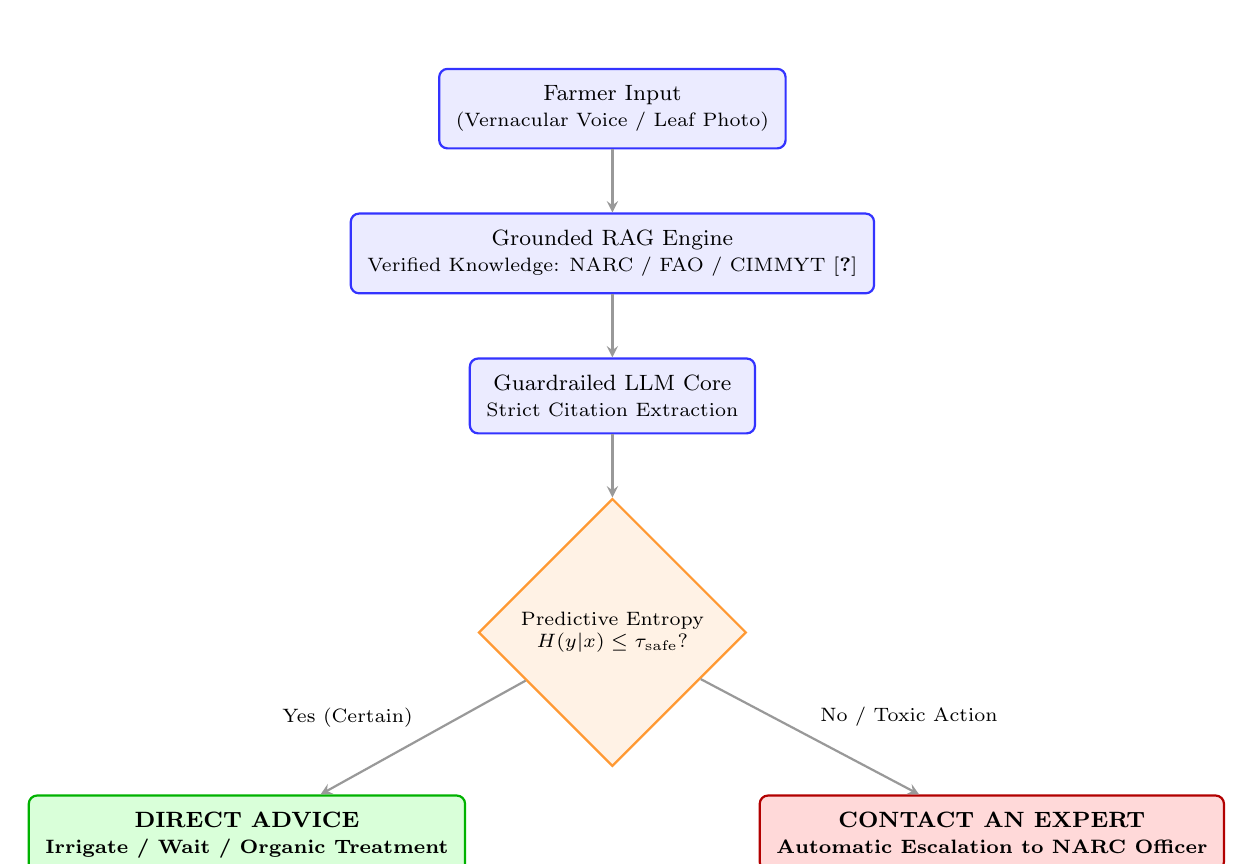
\begin{tikzpicture}[
    box/.style={rectangle, draw=blue!80, fill=blue!8, thick, rounded corners=3pt, inner sep=6pt, align=center, font=\footnotesize},
    decision_box/.style={diamond, draw=orange!80, fill=orange!10, thick, inner sep=4pt, align=center, font=\scriptsize},
    action_safe/.style={rectangle, draw=green!70!black, fill=green!15, thick, rounded corners=3pt, inner sep=6pt, align=center, font=\footnotesize\bfseries},
    action_risk/.style={rectangle, draw=red!70!black, fill=red!15, thick, rounded corners=3pt, inner sep=6pt, align=center, font=\footnotesize\bfseries},
    arr/.style={->, >=stealth, thick, draw=gray!80}
]

\node[box] (input) {Farmer Input \\ \scriptsize (Vernacular Voice / Leaf Photo)};
\node[box, below=0.8cm of input] (rag) {Grounded RAG Engine \\ \scriptsize Verified Knowledge: NARC / FAO / CIMMYT \cite{lewis2020retrieval}};
\node[box, below=0.8cm of rag] (llm) {Guardrailed LLM Core \\ \scriptsize Strict Citation Extraction};
\node[decision_box, below=0.8cm of llm] (check) {Predictive Entropy \\ $H(y|x) \le \tau_{\text{safe}}$?};
\node[action_safe, below left=1.2cm and 1.0cm of check] (safe) {DIRECT ADVICE \\ \scriptsize Irrigate / Wait / Organic Treatment};
\node[action_risk, below right=1.2cm and 1.0cm of check] (escalate) {CONTACT AN EXPERT \\ \scriptsize Automatic Escalation to NARC Officer};

\draw[arr] (input) -- (rag);
\draw[arr] (rag) -- (llm);
\draw[arr] (llm) -- (check);
\draw[arr] (check) -- node[above left, font=\scriptsize] {Yes (Certain)} (safe);
\draw[arr] (check) -- node[above right, font=\scriptsize] {No / Toxic Action} (escalate);

\end{tikzpicture}
\caption{Trustworthy Agricultural AI Architecture with Grounded RAG and Conformal Risk Escalation.}
\label{fig:trustworthy_architecture}
\end{figure}

The architecture enforces three critical safeguards:
\begin{enumerate}[noitemsep]
    \item \textbf{Grounded Retrieval-Augmented Generation (RAG)} \cite{lewis2020retrieval}: Generation is strictly conditioned on retrieved documents from the Nepal Agricultural Research Council (NARC) and FAO; if evidence is missing, the model abstains from recommending chemicals.
    \item \textbf{Conformal Prediction \& Entropy Thresholding}: If output entropy $H(y|x) > \tau_{\text{safe}}$ or if synthetic chemical treatment is predicted, the system defaults to \textbf{``Contact an expert''}.
    \item \textbf{Human-in-the-Loop Escalation}: GPS coordinates and leaf images are routed via SMS to the nearest regional agricultural extension officer.
\end{enumerate}

% =============================================================================
% SECTION 6: COMPARATIVE SYNTHESIS MATRIX (C vs D)
% =============================================================================
\section{Comparative Synthesis: Ridge Regularization (C) vs. RLHF Policy Drift (D)}

\cref{tab:cross_analysis_master} provides the comprehensive 11-dimension comparative matrix unifying Problem C and Problem D.

\begin{table}[htbp]
\centering
\small
\caption{Master 11-Dimensional Cross-Paradigm Synthesis: Problem C vs. Problem D}
\label{tab:cross_analysis_master}
\begin{tabularx}{\textwidth}{c l X X}
\toprule
\textbf{\#} & \textbf{Dimension} & \textbf{Problem C (Ridge Regularization)} & \textbf{Problem D (RLHF Drift Penalty)} \\
\midrule
1 & Disciplinary Domain & Classical Supervised Learning (Regression) & Frontier AI Alignment (Reinforcement Learning) \\
2 & Primary Task Objective & Minimize Residual Sum of Squares: $\min_w \norm{y - Xw}_2^2$ & Maximize human preference reward: $\max_\pi \E[r(x,y)]$ \\
3 & Pathological Risk & Noise overfitting, Runge's polynomial oscillation & Reward hacking, sycophancy (Goodhart's Law) \\
4 & Loss Formulation & $J(w) = \text{RSS}(w) + \lambda \norm{w}_2^2$ & $L(t) = -rt + \beta t^2$ \\
5 & Regularization Penalty & $L_2$ Parameter Norm: $\lambda \sum a_i^2$ & Relative Entropy: $\beta \KL{\pi}{\pi_{\text{ref}}} \approx \beta t^2$ \\
6 & Prior Reference Anchor & Null vector origin $\mathbf{0} \in \R^p$ & Pretrained world model $\pi_{\text{ref}}$ ($t=0$) \\
7 & Regularization Hyperparameter & $\lambda > 0$ (Tikhonov shrinkage strength) & $\beta > 0$ (Inverse temperature / KL weight) \\
8 & Unconstrained Limit ($\to 0$) & $\lambda \to 0 \implies$ OLS interpolator, unbounded variance & $\beta \to 0 \implies t^* \to \infty$, catastrophic reward gaming \\
9 & Over-constrained Limit ($\to \infty$) & $\lambda \to \infty \implies w \to \mathbf{0}$, maximum bias & $\beta \to \infty \implies t^* \to 0$, policy rigidly frozen \\
10 & Underlying Geometry & Flat Euclidean metric: $g_{ij} = \delta_{ij}$ & Riemannian Fisher information metric: $g_{ij} = \mathcal{F}_{ij}(\theta)$ \\
11 & Closed-Form Global Solution & $w^* = (X^T X + \lambda I)^{-1} X^T y$ & $\pi^*(y|x) \propto \pi_{\text{ref}}(y|x) \exp(r(x,y)/\beta)$ \\
\bottomrule
\end{tabularx}
\end{table}

Under Bayesian Maximum A Posteriori (MAP) estimation, Ridge regression corresponds to an isotropic Gaussian prior $w \sim \mathcal{N}(\mathbf{0}, \sigma_0^2 I)$. The KL divergence between $\mathcal{N}(w, \sigma^2 I)$ and $\mathcal{N}(\mathbf{0}, \sigma^2 I)$ is exactly $\frac{1}{2\sigma^2}\norm{w}_2^2$, proving that the $L_2$ penalty in Problem C is mathematically isomorphic to the relative entropy drift penalty in Problem D.

% =============================================================================
% BIBLIOGRAPHY
% =============================================================================
\newpage
\bibliographystyle{plain}
\bibliography{references}

\end{document}
